\documentclass{article}
% \usepackage{xeCJK}
\usepackage{amsmath}
\usepackage{amssymb}
\usepackage{mathrsfs}
\usepackage{xcolor}
\usepackage{bm}
\usepackage{hyperref}
\usepackage{graphicx}
\usepackage{subcaption}
\usepackage{float}
\usepackage{multicol}
\usepackage[ruled,linesnumbered]{algorithm2e}

\setlength{\parindent}{2em}
\usepackage{geometry}
\geometry{a4paper, left=2.54cm, right=2.54cm, top=3.18cm, bottom=3.18cm}

% 设置文章行距
% \renewcommand{\baselinestretch}{1.5}

% 定义引用格式
\hypersetup{
    colorlinks=true,
    linkcolor=blue,
    urlcolor=blue,
    citecolor=blue,
    linkbordercolor=white
}

\title{\textbf{Self-organized Chiral Swarmalators}}
\author{Yichen Lu}

\begin{document}

\maketitle

\tableofcontents

\newpage
\section{Models}
\subsection{Definitions}
\subsubsection{Self-propelled dynamics}

\begin{subequations}
    \begin{align}
    \dot{x}_i&=v\cos \theta _i\;,
    \\
    \dot{y}_i&=v\sin \theta _i\;,
    \end{align}
    \label{eq:dotxy}
\end{subequations}

\subsubsection{Phase coupling dynamics}
\begin{itemize}
    \item Additive coupling: 
    \begin{equation}
        \label{eq:additionalCouplingDotTheta}
        \dot{\theta}_i=\omega _i+K\sum_{j=1}^{N}f\left( r_{ij} \right)\sin \left( \theta _j-\theta _i+\alpha \right)\;,
    \end{equation}
    \item Mean-field coupling by oscillator number:
    \begin{equation}
        \label{eq:swarmalatorDotTheta}
        \dot{\theta}_i=\omega _i+\frac{K}{N}\sum_{j=1}^N{f}\left( r_{ij} \right) \sin \left( \theta _j-\theta _i+\alpha \right) \;,
    \end{equation}
    which is similar to the swarmalator model.
    % \item Mean-field coupling by oscillator density:
    % \begin{equation}
    %     \dot{\theta}_i=\omega _i+\frac{KL^2}{\pi d_{0}^{2}N}\sum_{j=1}^N{f}\left( r_{ij} \right) \sin \left( \theta _j-\theta _i+\alpha \right) \;,
    % \end{equation}
    % where $d_0$ is the radius of the interaction circle.
\end{itemize}
Here,  $f\left( r_{ij} \right)$ is a function of $r=\left| \mathbf{r}_i-\mathbf{r}_j \right|$, and $K$ is the coupling strength. 
The function $f\left( r \right)$ can be defined as
\begin{enumerate}
    \item $f_H\left( r \right)=H\left( d_0-r \right),\;r_0>0$;
    \item $f_E\left( r \right)=e^{-\frac{r}{d_0}},\;r_0>0$.
\end{enumerate}
The natural frequencies $\omega_i$ are distributed with following two cases:
\begin{enumerate}
    \item \textbf{Single-chiral swarmalators:} The natural frequencies $\omega_i$ are distributed in $U\left( \omega _{\min},\omega _{\max} \right)$ for all swarmalators and $\omega _{\min}\omega _{\max}>0$.
    
    \item \textbf{Double-chiral swarmalators:} The frequencies are distributed in two symmetric uniform distributions, representing two types of chirality. Exactly half of the swarmalators have natural frequencies $\omega_i \sim U\left( \omega _{\min},\omega _{\max} \right)$ and the other half have natural frequencies $\omega_i \sim U\left( -\omega _{\max},-\omega _{\min} \right)$.
\end{enumerate}

\subsubsection{Chemical field}
\noindent{\textbf{Same chemical product}}

\noindent Consider a chemical field $c\left( \mathbf{r},t \right)$ that is produced by the ensemble of ‘signalling’ rotors. Swarmalators interact with the chemical field and move towards the regions with higher concentration, which can be described by the following equation:
\begin{equation}
    \dot{\theta}_i=\omega _i+\beta _R\mathbf{p}_i\times \nabla c+\frac{K}{N}\sum_{j=1}^N{f}\left( r_{ij} \right) \sin \left( \theta _j-\theta _i+\alpha \right) \;,
\end{equation}
where $\beta _R$ denotes the ‘chemotactic’ coupling strength and $\mathbf{p}_i=(\cos \theta _i,\sin \theta _i)$ is the unit vector pointing in the direction of the $i$-th swarmalator. Here, we used the notation $\mathbf{a}\times\mathbf{b}=a_1 b_2-a_2 b_1$.
This field evolves as
\begin{equation}
    \dot{c}=\frac{k_0}{N}\sum_{j=1}^N{f\left( \left| \mathbf{r}-\mathbf{r}_j \right| \right)}-k_dc+D_c\nabla ^2c+\varepsilon \left( c_0-c \right) ^3\;,
\end{equation}
where $k_0$ is the production rate, $k_d$ is the decay rate, $D_c$ is the diffusion coefficient, and the term proportional to $\varepsilon$ prevents unlimited growth of $c$ in case of linear instability.

% \noindent{\textbf{Activator \& inhibitor chemical products}}

% Inspired by \textit{Gray-Scott}

% \begin{equation}
%     \dot{\theta}_i=\omega _i+\beta _R\mathbf{p}_i\times \nabla \left( u+v \right) +\frac{K}{N}\sum_{j=1}^N{f}\left( r_{ij} \right) \sin \left( \theta _j-\theta _i \right) \;,
% \end{equation}

% \begin{subequations}
%     \begin{align}
%         \dot{u}&=\frac{k_0}{N}\sum_{j\in C_+}{f\left( \left| \mathbf{r}-\mathbf{r}_j \right| \right)}-uv^2-k_du+D_u\nabla ^2u+\varepsilon \left( u_0-u \right) ^3\;,
%         \\
%         \dot{v}&=\frac{k_0}{N}\sum_{j\in C_-}{f\left( \left| \mathbf{r}-\mathbf{r}_j \right| \right)}+uv^2-k_dv+D_v\nabla ^2v+\varepsilon \left( v_0-v \right) ^3\;,
%     \end{align}
% \end{subequations}

\noindent{\textbf{Two Species}}

\begin{subequations}
    \begin{align}
        \dot{\mathbf{r}}_i&=v\mathbf{p}_i\\
        \dot{\theta}_i&=\omega _i+\beta _{i}^{u}\mathbf{p}_i\times \nabla u+\beta _{i}^{v}\mathbf{p}_i\times \nabla v+\frac{K}{N}\sum_{j=1}^N{f}\left( \left| \mathbf{r}_j-\mathbf{r}_i \right| \right) \sin \left( \theta _j-\theta _i \right) \;,\\
        \dot{u}&=k_0\sum_{j\in S_+}{\delta \left( \mathbf{r}-\mathbf{r}_{j} \right)}-k_du+D_u\nabla ^2u\;,\\
        \dot{v}&=k_0\sum_{j\in S_-}{\delta \left( \mathbf{r}-\mathbf{r}_{j} \right)}-k_dv+D_v\nabla ^2v\;,
    \end{align}
\end{subequations}

\subsubsection{Order Parameters}
Some order parameters can be introduced to measure the level of spatiotemporal coordinations among swarmalators and distinguish the different collective states of the system. Firstly, the usual order parameter to measure the global phase synchronization among swarmalators can be defined as the following complex function:
\begin{equation}
    Z\left( t \right) =R\left( t \right) \mathrm{e}^{\textrm{i}\psi(t)}=\frac{1}{N}\sum_{j=1}^N{\mathrm{e}^{\textrm{i}\theta _j(t)}}\;,
\end{equation}
where $\textrm{i}=\sqrt{-1}$. The degree modulus $R(t)=\left|Z(t)\right|$ is the absolute value of the mean of the complex numbers $e^{\textrm{i}\theta _i}$, which can be interpreted as the absolute value of the mean normalized velocity of all swarmalators. When $R\approx 1$, swarmalators are fully phase synchronized, and when $R\approx0$, swarmalators are phase incoherent.

The order parameter $R$ is not enough to measure the emergence of partial clustered phase synchronization of swarmalators. Therefore a local order parameter can be introduced to measure the clustered synchronization:
\begin{equation}
    Z_c^k (t) = R_c^k \left( t \right) \mathrm{e}^{\textrm{i}\psi_c^k (t)} =  \frac{1}{\left| C_k\left( t \right) \right|}\sum_{j\in C_k\left( t \right)}{\mathrm{e}^{\mathrm{i}\theta _j\left( t \right)}} \;,
\end{equation}
$N_c$ is the number of clusters, $C_k$ is the $k$-th cluster, and $\left| C_k \right|$ is the number of swarmalators in the $k$-th cluster (see the details of the determination of clusters in Appendix ). An averaged global order parameter can be further introduced as
\begin{equation}
    R_c\left( t \right) =\frac{1}{N_c\left( t \right)}\sum_{k=1}^{N_c\left( t \right)}{R^k_c (t)}\;.
\end{equation}
As the swarmalators within the $k$-th cluster are fully synchronized, $R_c^k\approx 1$, and therefore also globally $R_c\approx 1$.

Except the study for phase coherence, other order parameters can be defined to further describe the locking of the frequencies of swarmalators under the chiral condition. One first introduce a cluster frequency difference to measure the chiral synchronizability of swarmalators within a cluster as
\begin{equation}
    \Delta \Omega_c^k = \frac{1}{\left| C_k \right|^2}\sum_{i,j\in C_k}{\left( \left< \dot{\theta}_i \right> -\left< \dot{\theta}_j \right> \right) ^2} ,
    \label{eq:clusterfrequency}
\end{equation}
where $\left< \dot{\theta}_i \right>$ is the average phase velocity of the $i$-th cluster, which can be defined by
\begin{equation}
    \left< \dot{\theta}_i \right> =\lim_{T\rightarrow \infty} \frac{1}{T}\int_{t_0}^{t_0+T}{\dot{\theta}_i\left( t \right) \mathrm{d}t}\;.
    \label{eq:frequency}
\end{equation}
Then a global frequency difference of clusters is
\begin{equation}
    \Delta \Omega_c =\frac{1}{N_c}\sum_{k=1}^{N_c} {\Delta \Omega_c^k}\;.
    \label{eq:globalcluster}
\end{equation}
% Yichen: 暂时没有用到这个\Delta\Omega,所以先注释掉
% Of course it is natural to introduce a global frequency difference without the identification of multiple clusters as
% \begin{equation}
%     \Delta \Omega =\frac{1}{N^2}\sum_{i,j=1}^{N}{\left( \left< \dot{\theta}_i \right> -\left< \dot{\theta}_j \right> \right) ^2 }\;.
%     \label{eq:frequencydifference}
% \end{equation}
For any cluster $k$, one can assume that $\left< \dot{\theta}_i \right>\in \left[a, b\right]$. Then the expectation of $\Delta \Omega_c^k$ can be calculated as
\begin{equation}
    E\left( \Delta \Omega _{c}^{k} \right) =2E\left( \left< \dot{\theta}_i \right> ^2 \right) -2E\left( \left< \dot{\theta}_i \right> \left< \dot{\theta}_j \right> \right)\;.
\end{equation}
For different cases of bounds, the value is
\begin{equation}
    E\left( \Delta \Omega _{c}^{k} \right) \begin{cases}
        =0,&		ab\geqslant 0\\
        >0,&		ab<0\\
    \end{cases}
\end{equation}
Therefore, if $n\rightarrow\infty$ and the average phase velocities of swarmalators within the cluster are all positive, all negative, $\Delta \Omega _{c}^{k}\approx0$, and we name this case as the \textit{chirality-locked cluster}. Otherwise, $\Delta \Omega _{c}^{k}>0$. 
When $\Delta\Omega_c \approx 0$, the swarmalators will organize to form several clusters, within each cluster swarmalators are chirality-locked. 
% When $\Delta\Omega \approx 0$, all swarmalators are frequency locked. 
Note that chirality locking is different from phase locking, as the chirality-locked swarmalators can have different phase velocities, which also means that they can have different rotational radii. 
Obviously, chirality locking is a more loose condition than phase locking. 

All the above order parameters measure different aspects of coordination in the phases of swarmalators. Because the phase variable describes the alignment of a swarmalator, various synchrony states imply the motion alignment of swarmalators in the swarming dynamics. 
% In the following discussions, we will further define more order parameters that are necessary to depict the spatial swarming ordering. 
In the following discussions, we further define an order parameter to depict the spatial swarming ordering:
\begin{equation}
    \label{eq:relativeNumber}
    N_r\left( t \right) =\frac{1}{N}\frac{1}{N_c\left( t \right)}\sum_{k=1}^{N_c\left( t \right)}{\left| C_k\left( t \right) \right|}\;.
\end{equation}
$N_r$ is the relative number of swarmalators in the clusters, which measures the spatial condensation of swarmalators. When $N_r\approx 1$, swarmalators are fully spatially condensed, and when $N_r\approx 0$, swarmalators are spatially dispersed. 

\newpage
\section{Results}
\subsection{Signle-chiral Swarmalators}
\begin{figure}[H]
    \includegraphics[width=\textwidth]{./figs/MonoChiralPhaseDiagram.pdf}
    \caption{
        \label{fig:MonoPhaseDiagram} 
        Phase diagram and snapshots of mono-chiral swarmalators.
        \textbf{(a)} Phase diagram in the $(d_0$-$\lambda)$ plane. 
        % The boundaries between states are analytical approximations given by Section~\ref{sec:phaseDiagrams}.
        For the sake of clarity, the scale of $\lambda$ and $d_0$ is non-uniform.
        \textbf{(b)}, The snapshots of CS ($\lambda=0.08,\ d_0=0.1$). 
        \textbf{(c)}, DS ($\lambda=0.01,\ d_0=0.1$).
        \textbf{(d)}, CLS ($\lambda=0.3,\ d_0=1$).
        \textbf{(e)}, CLS ($\lambda=0.02,\ d_0=2$). The position and direction of each arrow are the instantaneous spatial position and phase of a swarmalator, respectively, and the color of the arrow denotes the corresponding natural frequency.
    }
\end{figure}

\begin{figure}[H]
    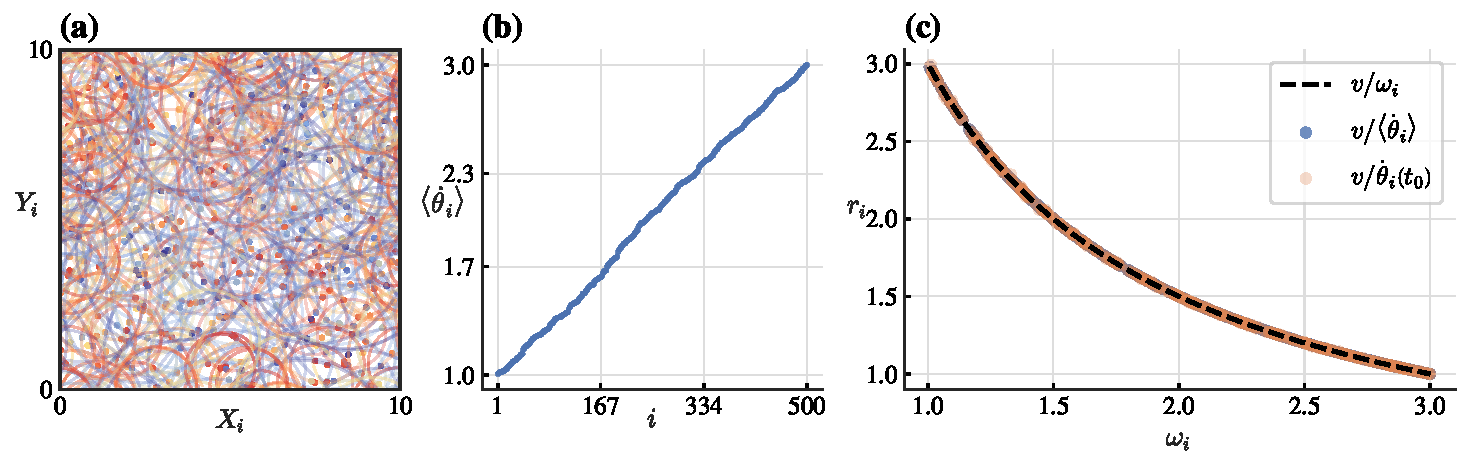
\includegraphics[width=\textwidth]{./figs/mono-DS.pdf}
    \caption{
        \label{fig:mono-DS} Swarming properties of DS for $\lambda =0.01$, $d_0 =0.1$. 
        \textbf{(a)}: The orbits and the instantaneous rotation centers $\left\{ \mathbf{c}_i (t)\right\}$ of swarmalators. The color denotes the natural frequency.
        \textbf{(b)}: The profile of the averaged frequencies $\langle \dot{\theta}_i \rangle$.
        \textbf{(c)}: The instantaneous rotation radii $ r_i^{eff}$ and the average rotation radii $v/\langle \dot{\theta}_i \rangle$ against the natural frequencies $\omega_i$. The black dashed line is the relation $r_i^0 = v/\omega_i$ for the uncoupled case.
    }
\end{figure}

\subsubsection{Spatial Clustering in Circling State}

\begin{figure}[H]
    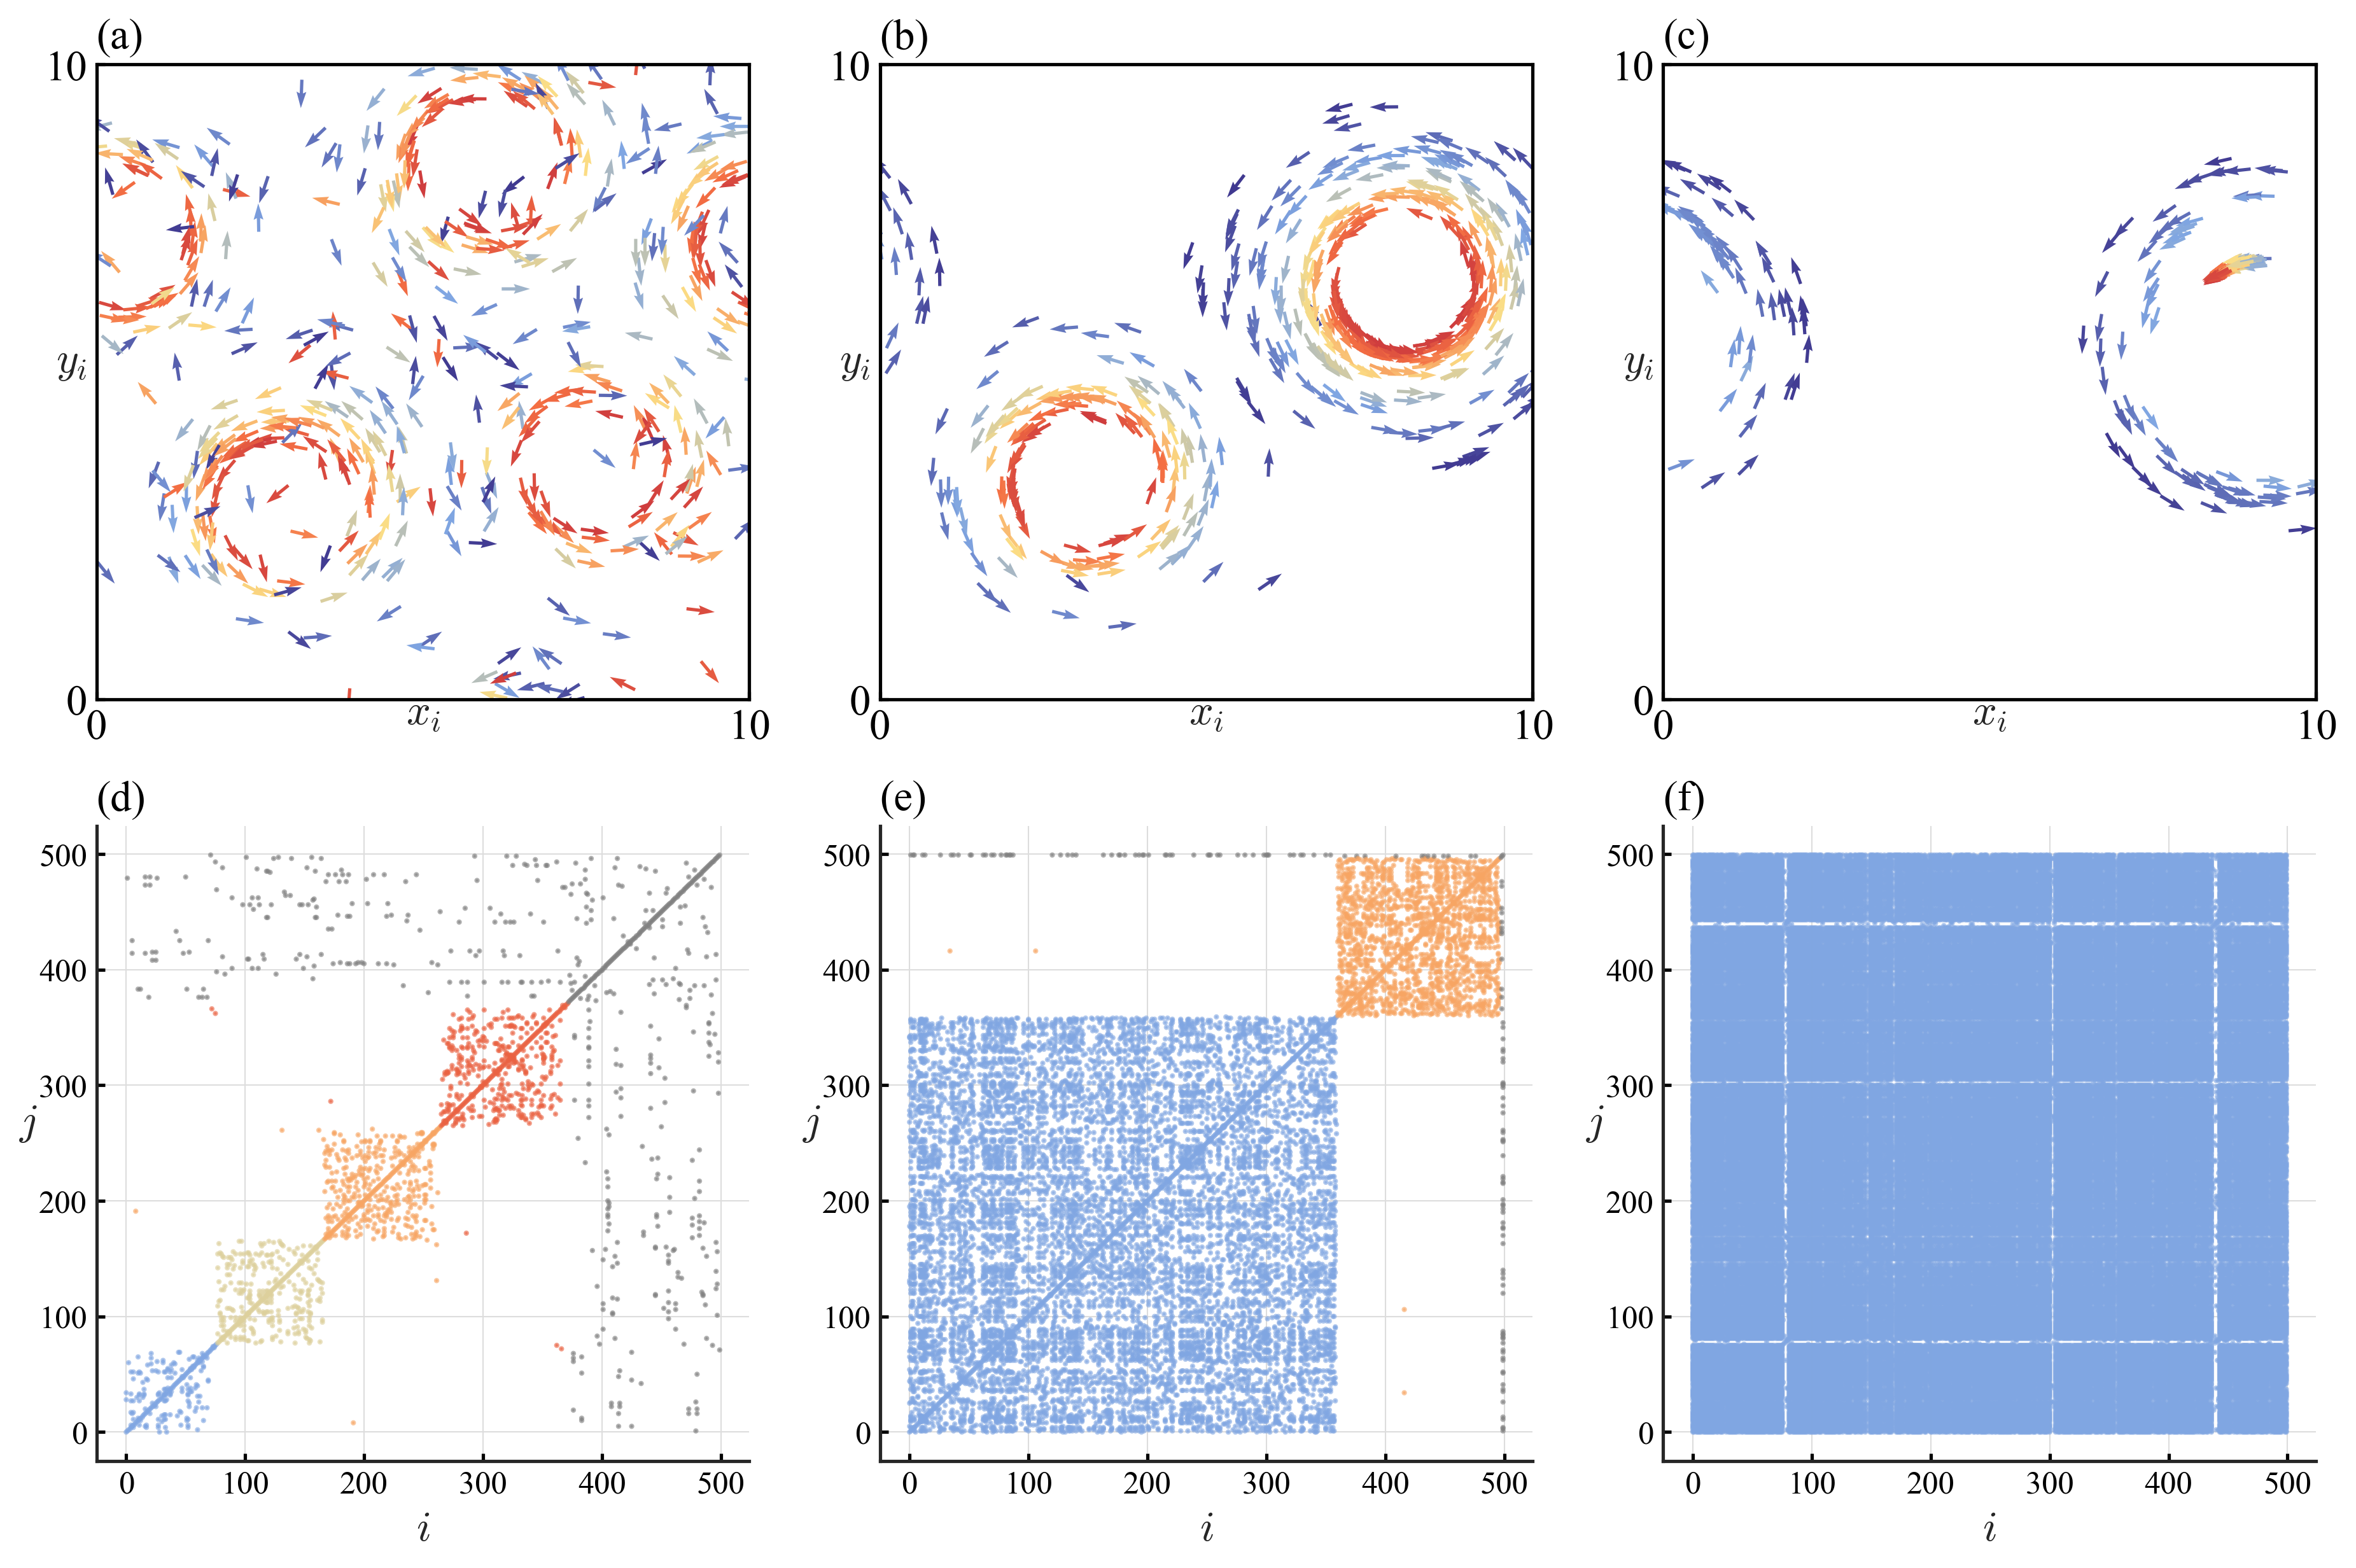
\includegraphics[width=\textwidth]{./figs/mono_CS_Aij.png}
    \caption{
        \label{fig:mono_CS_Aij}
        Spatial clustering in the circling state of single-chiral swarmalators. 
        Top row: snapshots of the spatial distribution of swarmalators. Bottom row: the adjacency matrix $A_{ij}$ of the network. 
        \textbf{(a, d)}: $(\lambda, d_0)=(0.01, 0.35)$.
        \textbf{(b, e)}: $(\lambda, d_0)=(0.01, 0.65)$.
        \textbf{(c, f)}: $(\lambda, d_0)=(0.01, 1.05)$.
        In \textbf{(d-f)}, only those elements $A_{ij}=1$ are plotted. The color of the matrix elements denotes different clusters, the gray elements represent the connections of the drifting swarmalators, and the white area represents the non-interacting region.
    }
\end{figure}

Sorting the swarmalators within each cluster by their standardized spatial angles, which are defined as
\begin{equation}
    \arctan \left( \frac{y_i-\bar{Y}_i}{x_i-\bar{X}_i} \right)\;,
\end{equation}
where 
\begin{equation}
    \left[ \begin{array}{c}
        \bar{Y}_i\\
        \bar{X}_i\\
    \end{array} \right] =\frac{1}{\left| C_k \right|}\sum_{i\in C_k}{\mathbf{c}_i}\;.
\end{equation}

\subsubsection{The Clustering State}
Swarmalators in a cluster are phase synchronized and exhibit a spatial rotation at a unified synchronous frequency $\omega_s$. By summing over Eq.~(\ref{eq:additionalCouplingDotTheta}), one gets the aligned frequency as
\begin{equation}
    \label{eq:clusterState}
    \begin{aligned}
        \omega _s&=\frac{1}{N_c}\sum_{i=1}^{N_c}{\omega _i}+\frac{\lambda}{N_c}\sum_{i=1}^{N_c}{\sum_{j=1}^{N_c}{A_{ij}\sin \left( \theta _j-\theta _i \right)}}\\
        &=\frac{1}{N_c}\sum_{i=1}^{N_c}{\omega _i}\;,\\
    \end{aligned}
\end{equation}
where $N_c$ is the number of swarmalators in the cluster.

% \begin{figure}[H]
%     \centering
%     \includegraphics[width=0.7\textwidth]{./figs/Radii.pdf}
%     \caption{
%         \label{fig:radiusOmega} The real-time rotation radii of swarmalators in DS (blue, $d_0=0.1$, $\lambda=0.01:0.02$) and CS (orange, $d_0=0.1$, $\lambda=0.03:0.04$). The real-time rotation radii are close to $v/\omega_i$. 
%     }
% \end{figure}

% \begin{equation}
%     \begin{aligned}
%         X_i\left( t \right) &=x_i\left( t \right) -\frac{v}{\dot{\theta}_i\left( t \right)}\sin \theta _i\left( t \right)\;,\\
%         Y_i\left( t \right) &=y_i\left( t \right) +\frac{v}{\dot{\theta}_i\left( t \right)}\cos \theta _i\left( t \right)\;,\\
%     \end{aligned}
% \end{equation}

% \begin{figure}[H]
%     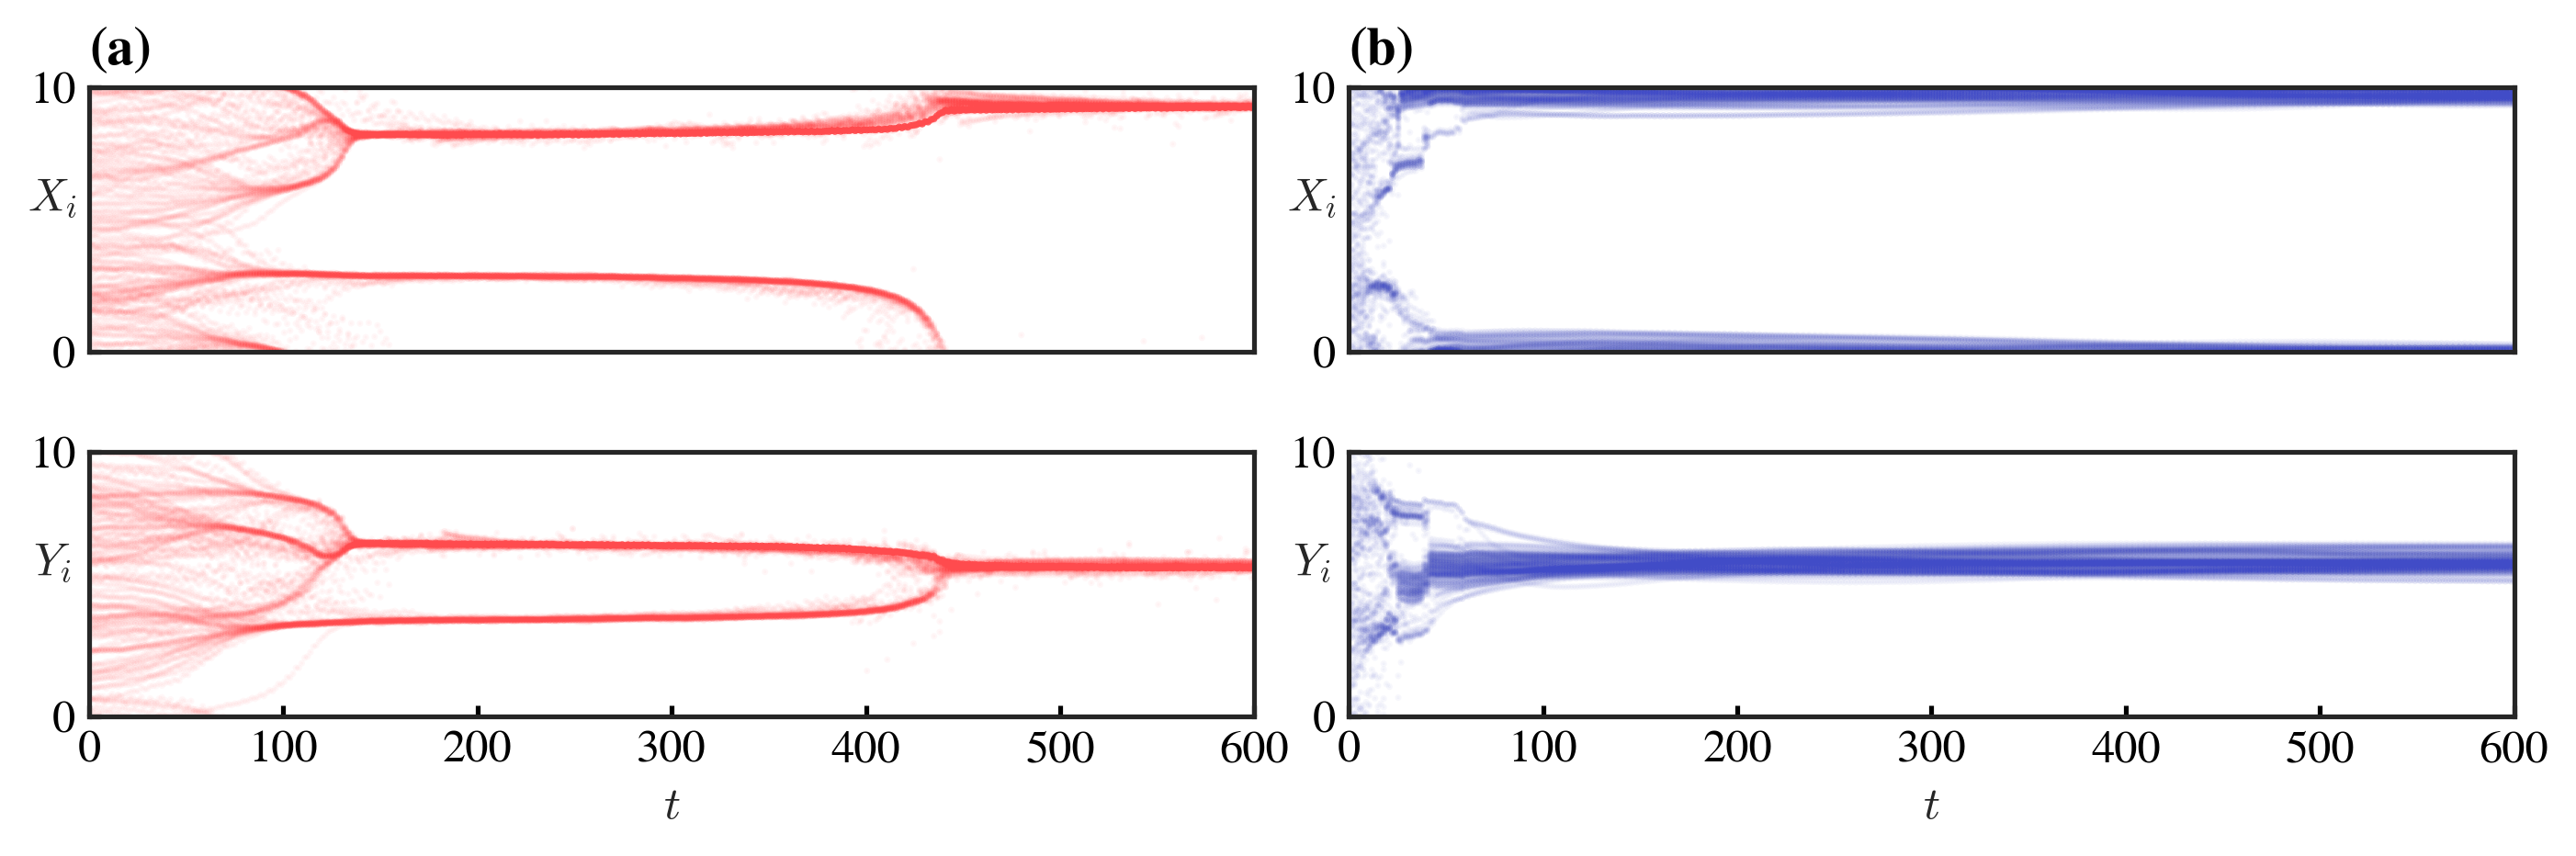
\includegraphics[width=\textwidth]{./figs/monoCentersPosition.png}
%     \caption{
%         \label{fig:monoCentersPosition} Scatter plot of the real-time centers of mono-chiral swarmalators.
%         \textbf{(a)}, centers position of CS ($\lambda=0.01$, $d_0=1$). 
%         \textbf{(b)}, centers position of CLS ($\lambda=0.045$, $d_0=1.05$). 
%         The color of the points denotes the corresponding natural frequency.
%     }
% \end{figure}

% \begin{figure}[H]
%     \centering
%     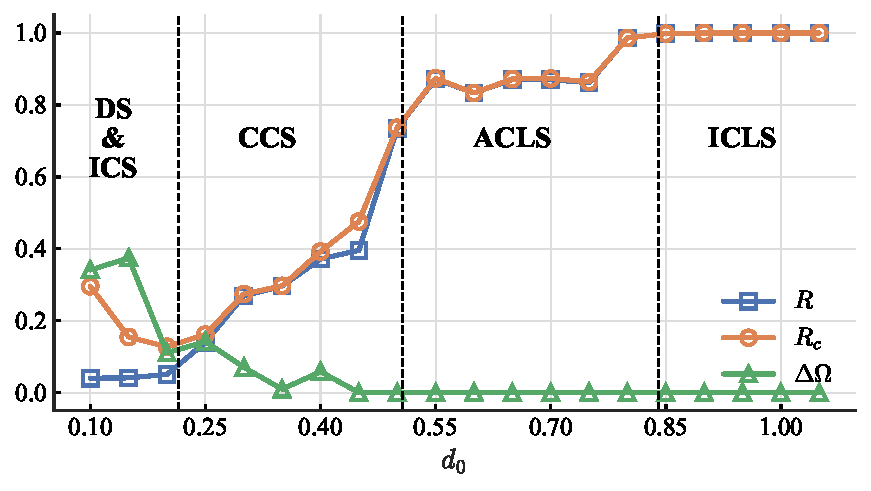
\includegraphics[width=0.7\textwidth]{./figs/monoOpPlot.pdf}
%     \caption{
%         \label{fig:monoOpPlot} Order parameters vary against $\lambda$ and $d_0$. 
%         \textbf{(a)}, $d_0=0.02$.
%         \textbf{(b)}, $\lambda=0.3$.
%         Blue, orange, green lines represent order parameters respectively for $R$, $R_c$ and $\Delta \Omega$.
%     }
% \end{figure}

% \subsection{Chiral Swarmalators}
% \begin{figure}[H]
%     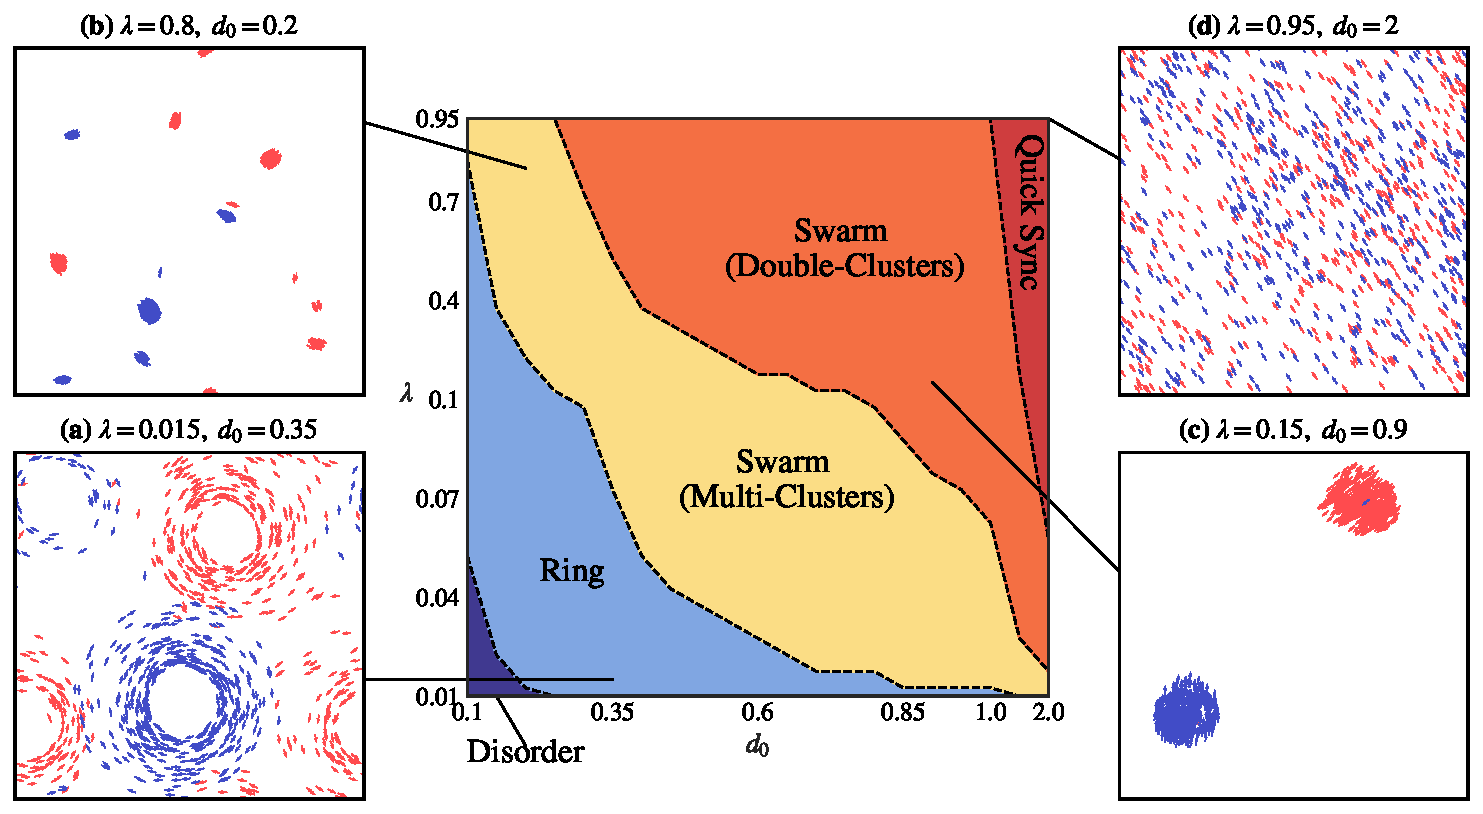
\includegraphics[width=\textwidth]{./figs/phaseDiagram.pdf}
%     \caption{
%         \label{fig:phaseDiagram} Phase diagram and snapshots of chiral swarmalators.
%         \textbf{(a)} Phase diagram in the $(d_0$-$\lambda)$ plane. The boundaries between states are analytical approximations given by Section~\ref{sec:phaseDiagrams}. 
%         For the sake of clarity, the scale of $\lambda$ and $d_0$ is non-uniform.
%         \textbf{(b)}, The snapshots of MCLS ($\lambda=0.4,\ d_0=0.3$). 
%         \textbf{(c)}, CS ($\lambda=0.02,\ d_0=0.4$).
%         \textbf{(d)}, ISS ($\lambda=0.95,\ d_0=2$).
%         \textbf{(e)}, DCLS ($\lambda=0.15,\ d_0=0.9$). 
%         Two types of chiral oscillators are represented by red ($\omega_i > 0$) and blue ($\omega_i < 0$) arrows, respectively. 
%     }
% \end{figure}

% \begin{figure}[H]
%     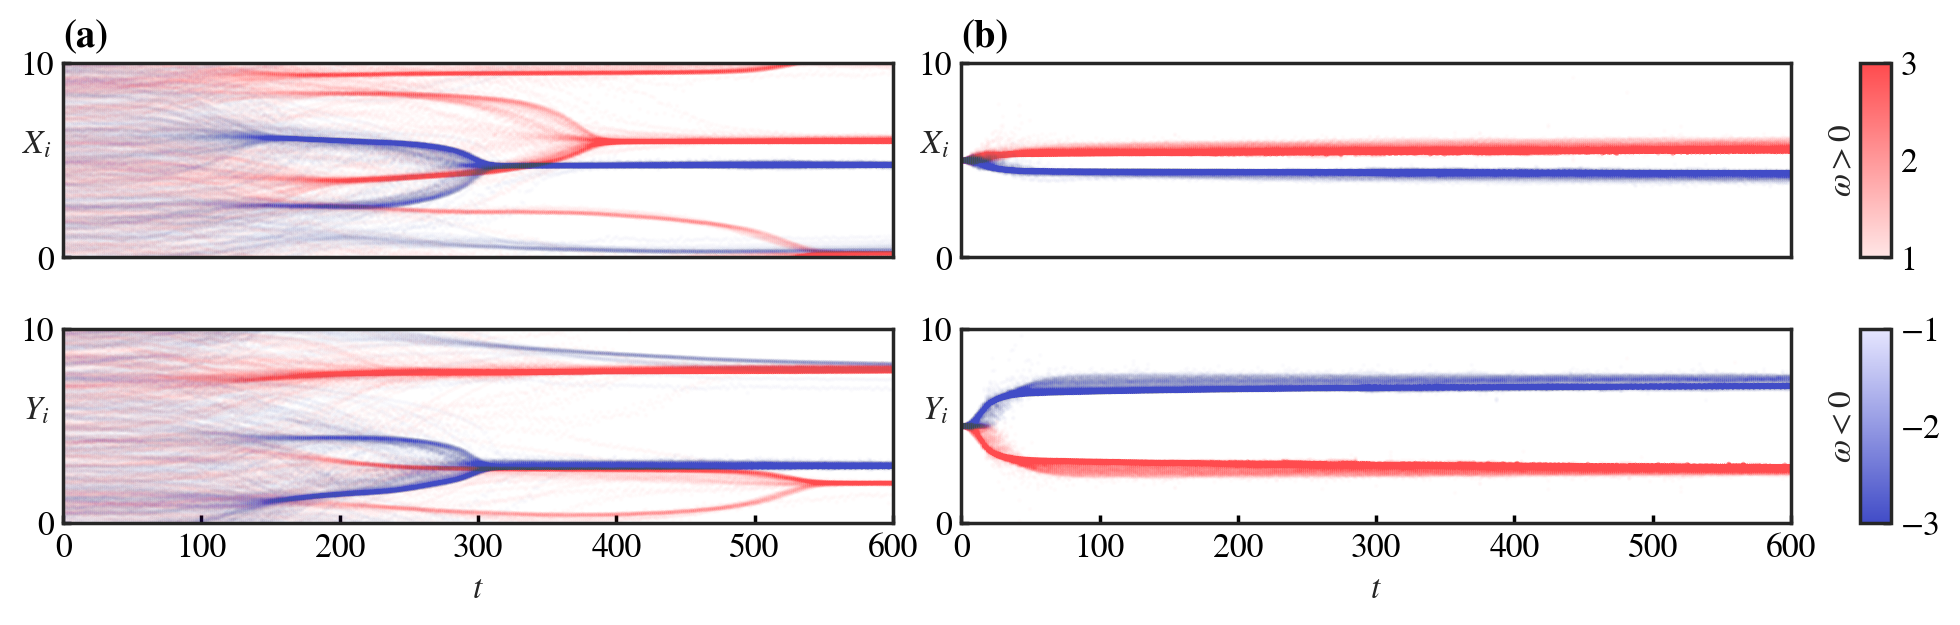
\includegraphics[width=\textwidth]{./figs/centersPosition.png}
%     \caption{
%         \label{fig:centersPosition} Scatter plot of the real-time centers of CS ($\lambda=0.02$, $d_0=0.4$).
%         \textbf{(a)}, behavior from random uniform initial condition. As time goes on, the centers of oscillators with the same chirality converge.
%         \textbf{(b)}, behavior from clustered initial condition. The centers of swarmalators are already clustered at a concentric ring.
%         The color of the points denotes the corresponding natural frequency.
%     }
% \end{figure}

% \begin{figure}[H]
%     \centering
%     \includegraphics[width=\textwidth]{./figs/Aij.png}
%     \caption{
%         \label{fig:Aij} The adjacency matrix $A_{ij}$ of chiral swarmalators. 
%         \textbf{(a)}, $A_{ij}$ of CS ($\lambda=0.02$, $d_0=0.4$).
%         \textbf{(b)}, $A_{ij}$ of CLS ($\lambda=0.15$, $d_0=0.9$).
%         The color of the point denotes the corresponding cluster index. No color means the $i$th swarmalator is not connected to $j$th swarmalator.
%     }
% \end{figure}

% \newpage
% \section{Mechanism of Condensation and Separation Dynamics}

% \begin{figure}[H]
%     \centering
%     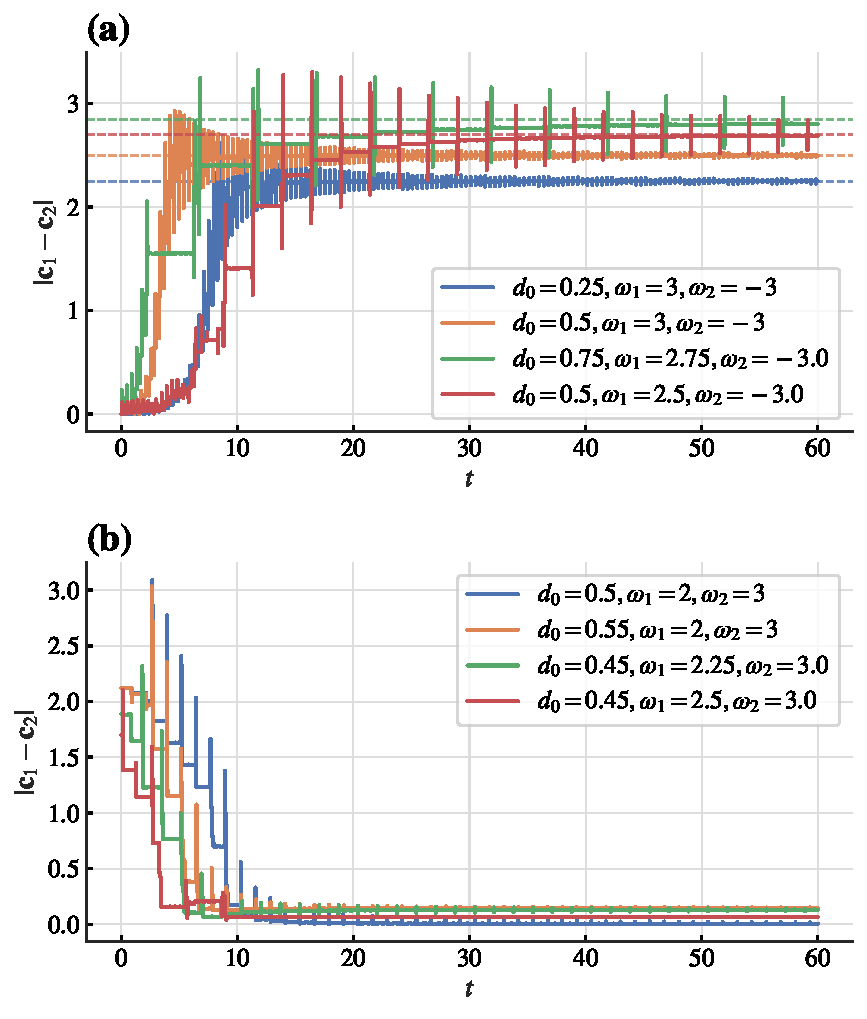
\includegraphics[width=0.7\textwidth]{./figs/2OsCenterDistance.pdf}
%     \caption{
%         \label{fig:2OsCenterDistance} The distance between the centers of two swarmalators ($\lambda=1$). 
%         \textbf{(a)}, The distance between the centers of two chiral swarmalators. The dashed line is the theoretical maximum distance.
%         \textbf{(b)}, The distance between the centers of two mono-chiral swarmalators.
%     }
% \end{figure}

% \newpage
% \section{Phase Diagrams and Critical Thresholds\label{sec:phaseDiagrams}}

\newpage
\begin{figure}[H]
    \centering
    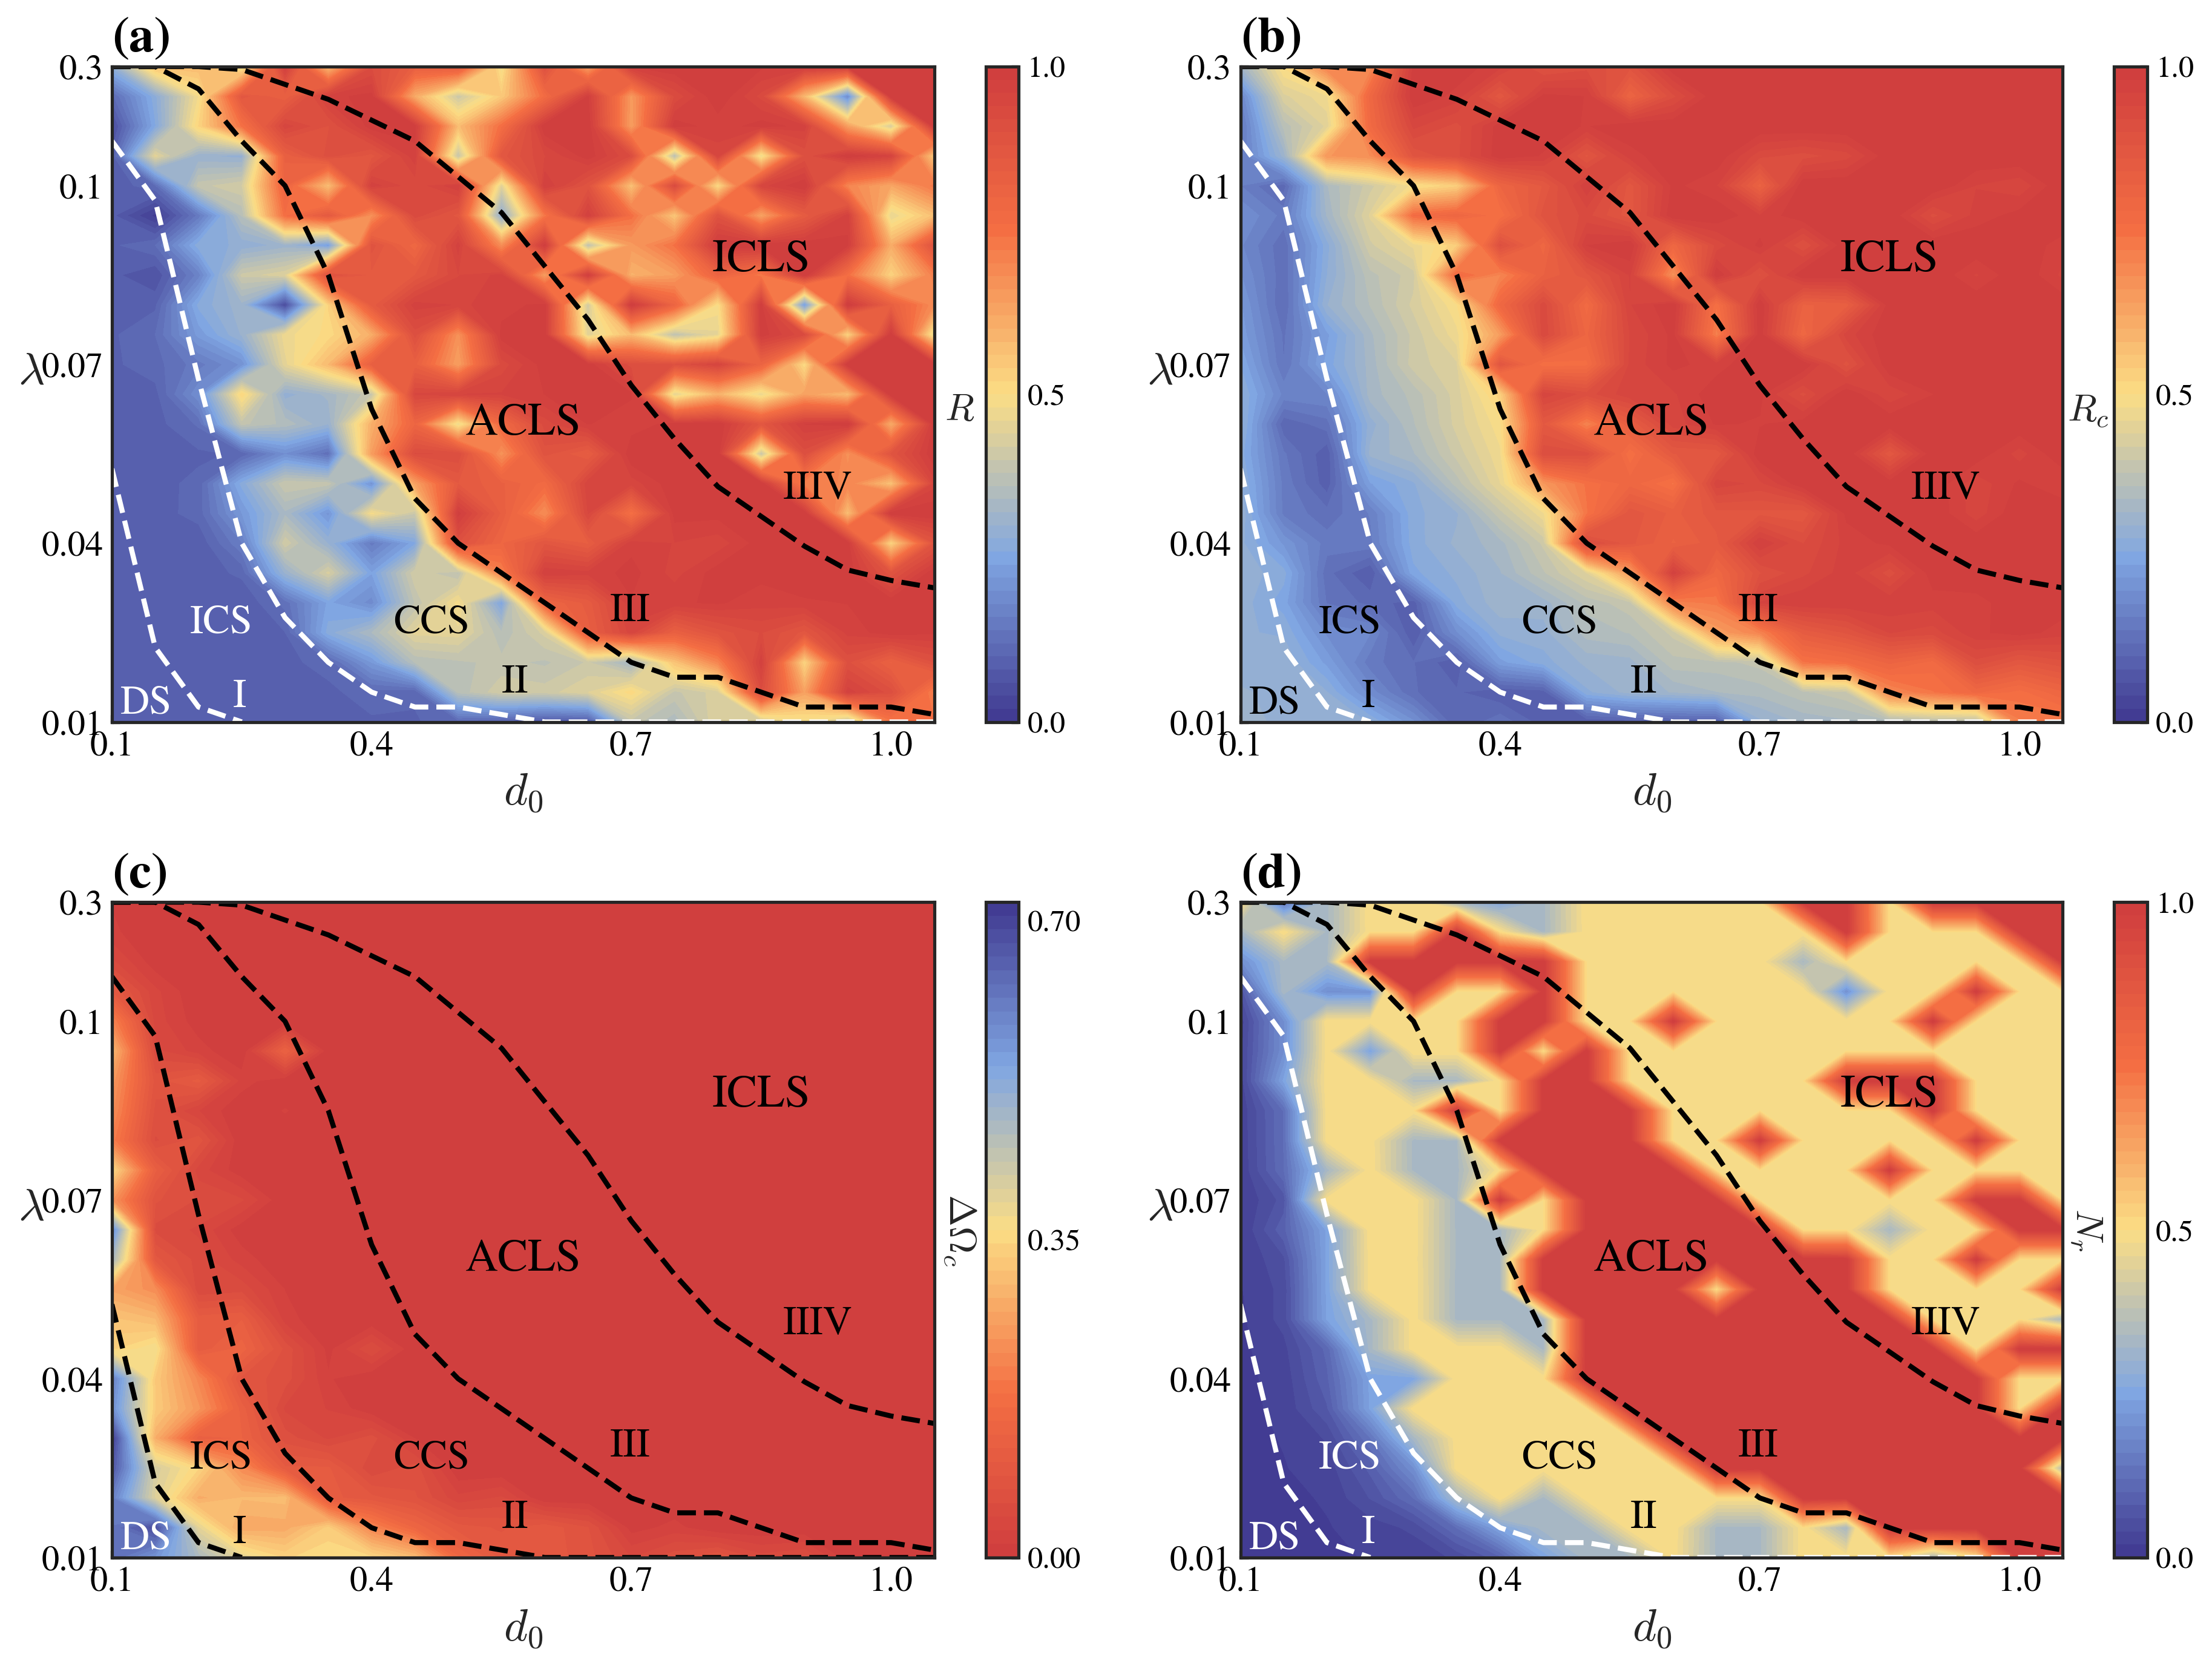
\includegraphics[width=0.75\textwidth]{./figs/monoOrderParam.png}
    \caption{
        \label{fig:monoOrderParam} Heatmaps for different order parameters of single-chiral swarmalators across the ($\lambda$, $d_0$) plane and the critical lines of the transitions between states.
        \textbf{(a)-(d)} correspond to the order parameters $R$, $R_c$, $\Delta \Omega_c$ and $N_r$, respectively.
        Different colors describe the amplitudes of different order parameters.
    }
\end{figure}

\begin{figure}[H]
    \centering
    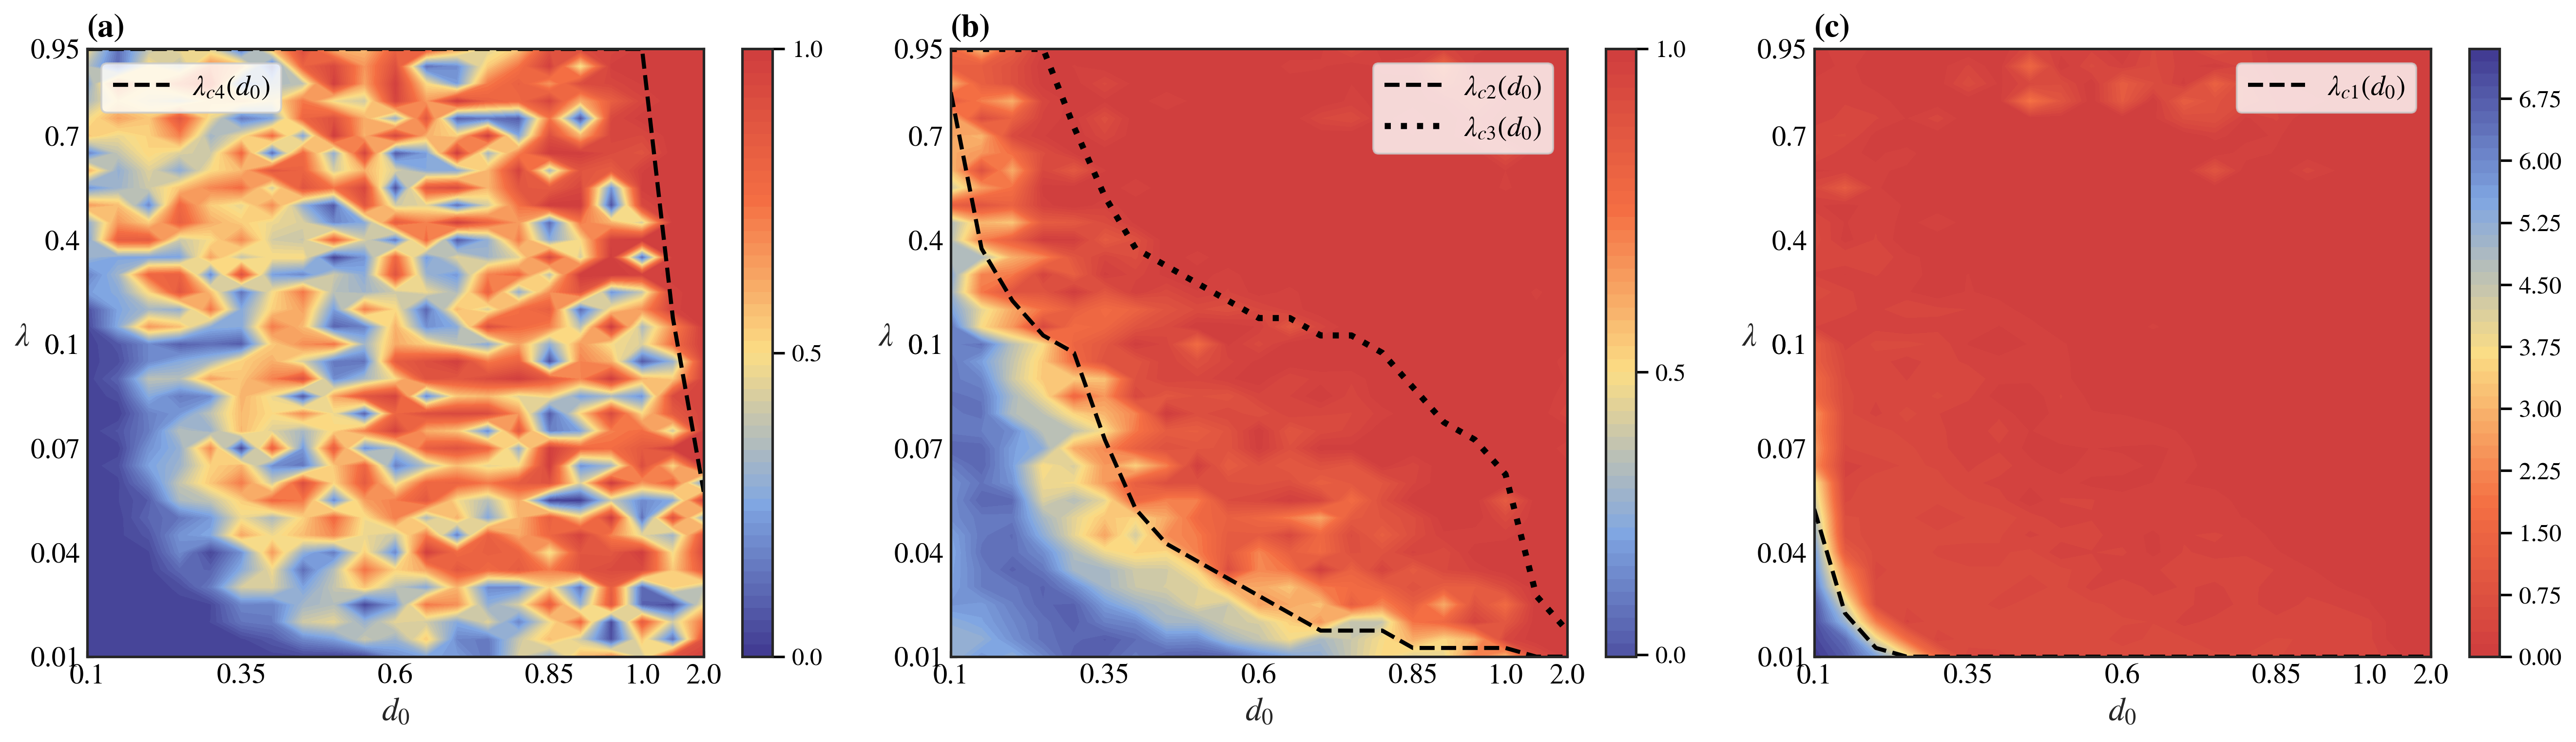
\includegraphics[width=0.75\textwidth]{./figs/orderParam.png}
    \caption{
        \label{fig:orderParam} Heatmaps for different order parameters of double-chiral swarmalators across the ($\lambda$, $d_0$) plane and the critical lines of the transitions between states.
        \textbf{(a)-(d)} correspond to the order parameters $R$, $R_c$, $\Delta \Omega_c$ and $N_r$, respectively.
        Different colors describe the amplitudes of various order parameters.
    }
\end{figure}

% \begin{figure}[H]
%     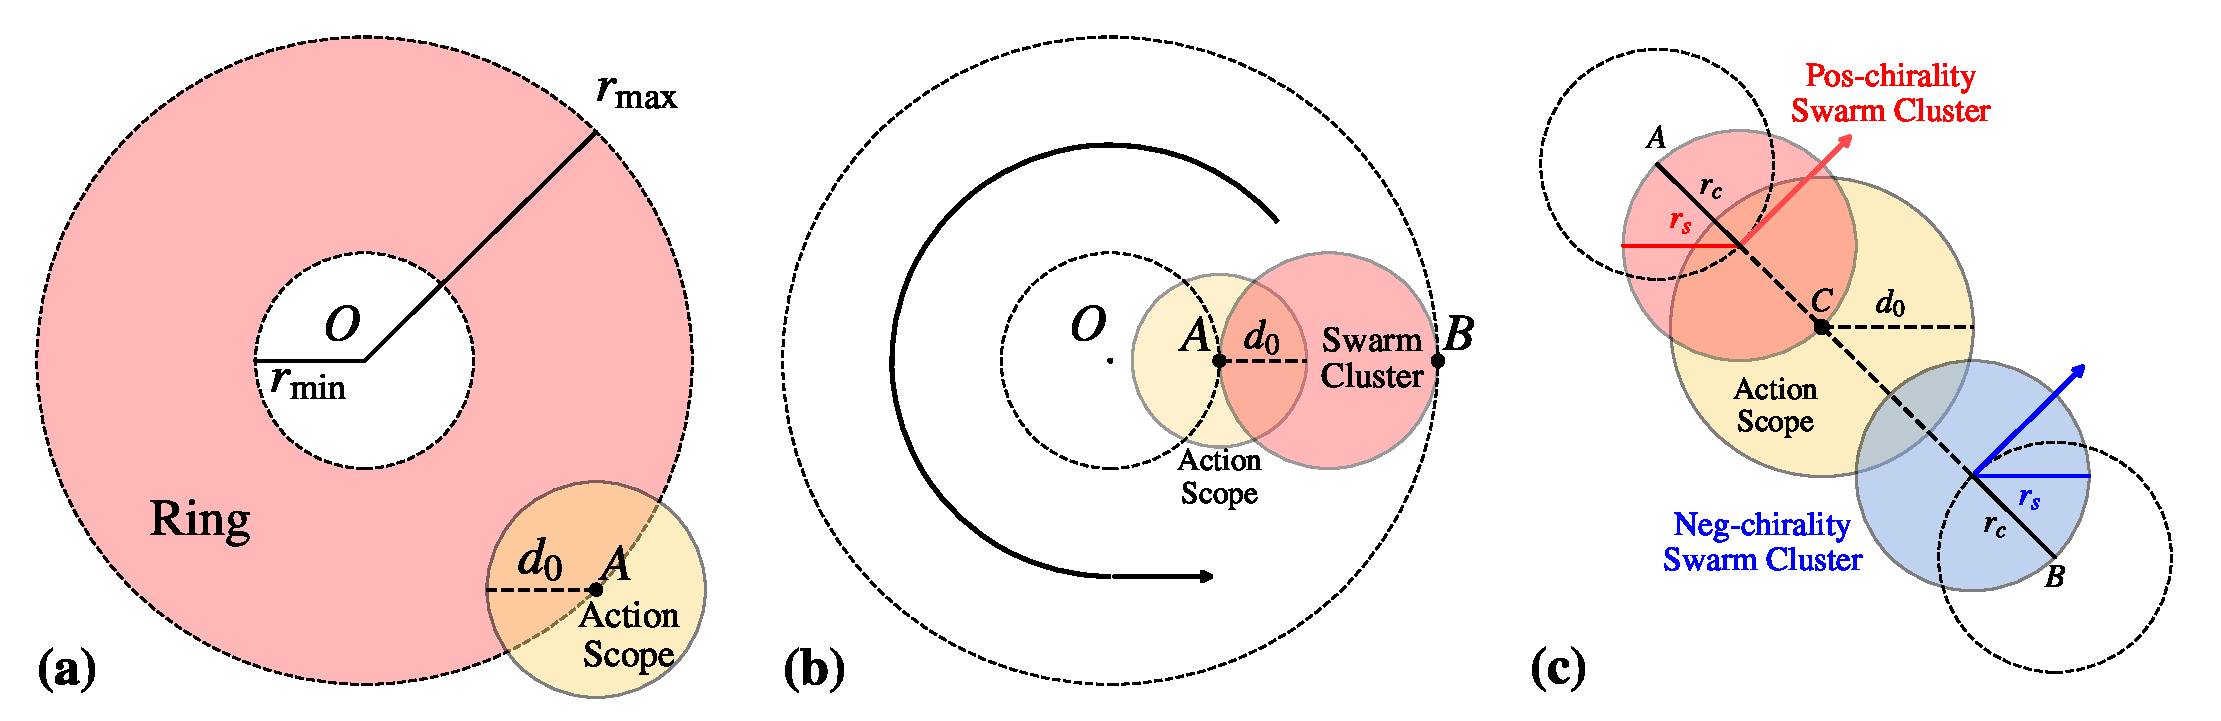
\includegraphics[width=\textwidth]{./figs/analyticalEps.pdf}
%     \caption{
%         \label{fig:analyticalEps}
%         The schematic plot of the analytical approximations.
%         \textbf{(a)}, The $1$st oscillator is at point $A$ which is on the outer edge of the ring, and the overlapping area of the yellow circle (action scope) and the red ring is $S_1\left( d_0 \right)$.
%         \textbf{(b)}, The $1$st oscillator is at point $A$ which is on the inner edge of the ring, and the overlapping area of the yellow circle (action scope) and the red ring is $S_2\left( d_0 \right)$.
%         \textbf{(c)}, The $1$st oscillator is at point $C$ which is on the edge of red circle, and the overlapping area of the yellow circle (action scope) and the blue circle is $S_3\left( d_0 \right)$.
%     }
% \end{figure}

% \begin{equation}
%     \begin{cases}
%         \lambda _{c1}=\frac{\pi \left( r_{\max}^{2}-r_{\min}^{2} \right) \left( \omega _{\max}-\omega _{\min} \right)}{N_{c}^{2}\left( d_{0}^{2}\frac{\alpha}{2}+r_{\max}^{2}\frac{\beta}{2}-r_{\max}d_0\sin \frac{\alpha}{2} \right)}\\
%         \beta =2\mathrm{arc}\cos \left( 1-\frac{d_{0}^{2}}{2r_{\max}^{2}} \right)\\
%         \alpha =\pi -\frac{\beta}{2}\\
%     \end{cases}\;.
% \end{equation}

% \begin{equation}
%     \begin{cases}
%         \lambda _{c2}=\frac{\pi r_{s}^{2}\left( \omega _{\max}-\omega _{\min} \right)}{N_S\left( d_{0}^{2}\frac{\alpha}{2}+r_{s}^{2}\frac{\beta}{2}-r_sd_0\sin \frac{\alpha}{2} \right)}\\
%         \beta =2\mathrm{arc}\cos \left( 1-\frac{d_{0}^{2}}{2r_{s}^{2}} \right)\\
%         \alpha =\pi -\frac{\beta}{2}\\
%         r_s=\frac{r_{\max}-r_{\min}}{2}\\
%     \end{cases}\;.
% \end{equation}

% \begin{equation}
%     \lambda _{c3}=\frac{L^2\left( \omega _{\max}-\omega _{\min} \right)}{N\pi d_{0}^{2}}\;.
% \end{equation}

% \begin{equation}
%     \begin{cases}
%         \lambda _{c4}=\frac{2\pi r_{s}^{2}\omega _{\max}}{N_c\left( \frac{\alpha}{2}r_{s}^{2}+\frac{\beta}{2}d_{0}^{2}-d_0r_d\sin \frac{\beta}{2} \right)}\\
%         r_d=\frac{L}{\sqrt{2}}-r_s-2r_c\\
%         \beta =2\mathrm{arc}\cos \frac{d_{0}^{2}+r_{d}^{2}-r_{s}^{2}}{2d_0r_d}\\
%         \alpha =2\mathrm{arc}\cos \frac{r_{s}^{2}+r_{d}^{2}-d_{0}^{2}}{2r_sr_d}\\
%     \end{cases}\;.
% \end{equation}

\section{Hydrodynamic Theory}

We replace the finite range alignment interaction by a pseudopotential ($\delta$-interaction) in the model:
\begin{equation}
    \label{eq:ourModel}
    \begin{aligned}
        \dot{\mathbf{r}}_i&=v\mathbf{p}_i\\
        \dot{\theta}_i&=\Omega _i+\lambda \sum_{j\ne i}{\delta}\left( \mathbf{r}_j-\mathbf{r}_i \right) \sin \left( \theta _j-\theta _i \right)\\
    \end{aligned}
\end{equation}
where $\mathbf{p}_i=(\cos\theta_i, \sin\theta_i)$. 
Assuming that we have $M$ species, consisting of $N_1, \dots, N_M$ particles with identical frequencies $\tilde{\Omega}_1, \dots, \tilde{\Omega}_M$ respectively, and that $N_1, \dots, N_M$ are all macroscopic in an area element over which macroscopic quantities (density, polarization) vary significantly, allows us to derive a continuum theory for the particle dynamics.
The combined probability density to find a particle of given species $j$ at position $\mathbf{r}$ with angle $\theta$ at time $t$ is given by
\begin{equation}
    \label{eq:combinedDensity}
    f^{\left( j \right)}\left( \mathbf{r},\theta ,t \right) =\sum_{i=1}^N{\delta \left( \mathbf{r}-\mathbf{r}_i\left( t \right) \right) \delta \left( \theta -\theta _i\left( t \right) \right) \delta _{\Omega _i,\tilde{\Omega}_j}}\;.
\end{equation}
A Boltzmann-like equation for the combined density $f^{\left( j \right)}$ can be derived:
\begin{equation}
    \label{eq:combinedDensityDynamics}
    \begin{aligned}
        \dot{f}^{(j)}(\mathbf{r},\theta,t)& = -\mathrm{Pe} \mathbf{p}\cdot\left[\nabla_\mathbf{r}f^{(j)}(\mathbf{r},\theta,t)\right]-\Omega_j\partial_\theta f^{(j)}(\mathbf{r},\theta,t)+\partial_\theta^2f^{(j)}(\mathbf{r},\theta,t) 
        \\
        &- g\partial_\theta\left[f^{(j)}(\mathbf{r},\theta,t)\int\mathrm{d}\theta^{\prime}\sin(\theta^{\prime}-\theta)\sum_{i=1}^Mf^{(i)}(\mathbf{r},\theta^{\prime},t)\right]-\partial_\theta\sqrt{2f^{(j)}(\mathbf{r},\theta,t)}\eta_j(\mathbf{r},\theta,t)
    \end{aligned}
\end{equation}
where $\eta_j$ represents spatiotemporal white noise with zero mean and unit-variance (the subscript $j$ denotes that the noise-realization of a given ensemble is individual for each species).

In the following, we focus on a mean-field description and neglect the (multiplicative) noise term in Eq.~\eqref{eq:combinedDensityDynamics}. 
Now transforming Eq.~\eqref{eq:combinedDensityDynamics} to Fourier space yields a hierarchy of dynamical equations for the Fourier modes
$
f_k^{(j)}(\mathbf{r}, t)=\int\mathrm{d}\theta f^{(j)}(\mathbf{r},\theta,t)\mathrm{e}^{\mathrm{i}k\theta}
$
and
$
2\pi f^{(j)}(\mathbf{r},\theta ,t)=\sum_{k=-\infty}^{\infty}{f_{k}^{(j)}}(\mathbf{r},t)\mathrm{e}^{-\mathrm{i}k\theta}
$,
reading
\begin{equation}
    \begin{aligned}
        \dot{f}_k^{(j)}(\mathbf{r},t)&=-\frac{\mathrm{Pe}}{2}\left[\partial_x\left(f_{k+1}^{(j)}+f_{k-1}^{(j)}\right)-\mathrm{i}\partial_y\left(f_{k+1}^{(j)}-f_{k-1}^{(j)}\right)\right]\\
        &+ \left(\mathrm{i}k\Omega_j-k^2\right)f_k^{(j)}+\frac{\mathrm{i}gk}{2\pi}\sum_{m=-\infty}^\infty f_{k-m}^{(j)}F_{-m}\sum_{i=1}^Mf_m^{(i)}
    \end{aligned}
\end{equation}

From here, some lengthy algebra leads us to the following closed set of equations of motion for the fields $\rho:=\rho^{(j)};\mathbf{w}:=\mathbf{w}^{(j)};\Omega:=\Omega_j$
\begin{equation}
    \label{eq:hydrodynamicEq}
    \begin{aligned}
        \dot{\rho} &= -\mathrm{Pe}\nabla\cdot\mathbf{w}\\
        \dot{\mathbf{w}} &= -\mathbf{w}+\sum_{i=1}^M\frac{g\rho}2\mathbf{w}^{(i)}-\frac{\mathrm{Pe}}2\nabla\rho+\frac{\mathrm{Pe}^2}{2b}\nabla^2\mathbf{w}-\frac{g^2}b\mathbf{w}\left(\sum_{i=1}^M\mathbf{w}^{(i)}\right)^2\\
        &+ \Omega\mathbf{w}_\perp+\frac{\mathrm{Pe}^2\Omega}{4b}\nabla^2\mathbf{w}_\perp-\frac{g^2\Omega\mathbf{w}_\perp}{2b}\left(\sum_{i=1}^M\mathbf{w}^{(i)}\right)^2+\mathcal{O}\left(\nabla\mathbf{w}^2\right)
    \end{aligned}
\end{equation}

where $b=2\left( 4+\Omega ^2 \right)$, $\mathbf{w}_{\bot}=\left( -w_y,w_x \right)$ and $\mathcal{O}\left(\nabla\mathbf{w}^2\right)$ represents all terms involving both derivatives and nonlinear terms in w of arbitrary species and are therefore irrelevant for both the set of possible uniform solutions and for the linear stability of unpolarized (disordered) phases and can therefore be neglected for our purposes.

\newpage
\section{Self-consistency Equation}

Inspired by global order parameter $R$, one can define the local order parameter $R_i$:
\begin{equation}
    \label{eq:localOrderParameter}
    R_{c}^{i}\mathrm{e}^{\mathrm{i}\psi _{c}^{i}}=\frac{1}{\left| C_i \right|}\sum_{j\in C_i}{\mathrm{e}^{\mathrm{i}\theta _j}}\;,
\end{equation}
where $C_i=\left\{ j\mid \Delta r_{ij}\le d_0 \right\}$. If the swarmalators in set $C_i$ are the initial to entry the coherent state, and other swarmalators are still in the incoherent state, then the $R_i$ will bifurcate from zero simultaneously with $R$ and $R_c$. Then the Eq.~\eqref{eq:swarmalatorDotTheta} can be rewritten as
\begin{equation}
    \label{eq:localDotTheta}
    \dot{\theta}_i=\omega _i+\frac{K}{N} \sum_{j\in C_i}{\sin \left( \theta _j-\theta _i \right)}\;.
\end{equation}
By introducing $\Sigma _2\left( d_0 \right) =\sum\nolimits_{j\in C_i}^{}{A_{ij}}=\left|C_i\right|$, Eq.~\eqref{eq:localOrderParameter} becomes 
\begin{equation}
    \frac{K\Sigma _2R_{c}^{i}}{N} \sin \left( \psi _{c}^{i}-\theta _i \right) =\frac{K}{N} \sum_{j\in C_k}{\sin \left( \theta _j-\theta _i \right)}
;.
\end{equation}
Then by introducing $\varphi _i=\theta _i-\bar{\omega}t=\theta_i-\psi _{c}^{i}$, where $\bar{\omega}=\sum_{j\in C_i}{\omega _j}/\left| C_i \right|$ is synchronous frequency of the swarmalators in $C_i$ given by Eq.~(\ref{eq:clusterState}), Eq.~(\ref{eq:localDotTheta}) can be recast as
\begin{equation}
    \label{eq:dotphi}
    \dot{\varphi}_i=\dot{\theta}_i-\bar{\omega}-\frac{K\Sigma _2R_{c}^{i}}{N} \sin \varphi _i\;.
\end{equation}

When $N\rightarrow \infty$, the mean field can be expressed by the distribution function as
\begin{equation}
    R_{c}^{i}\mathrm{e}^{\mathrm{i}\psi _{c}^{i}}=\mathrm{e}^{\mathrm{i}\bar{\omega}t}\int_0^{2\pi}{\int_{-\infty}^{\infty}{\mathrm{e}^{\mathrm{i}\varphi}}}P(\varphi ,\omega ,t)g(\omega )\mathrm{d}\omega \mathrm{d}\varphi\;.
\end{equation}

% \newpage
% \section{Appendix}

% \begin{figure}[H]
%     \centering
%     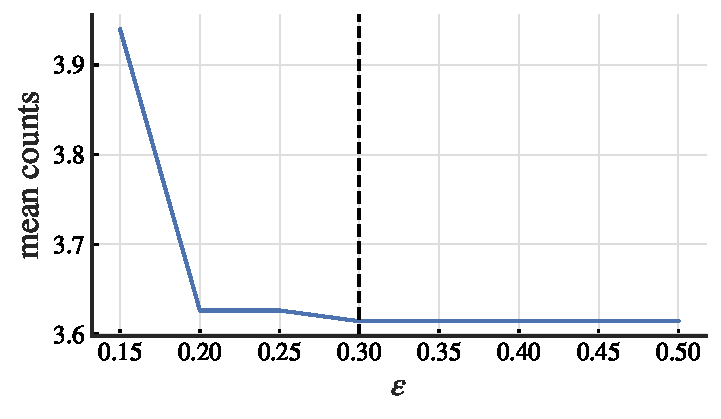
\includegraphics[width=0.7\textwidth]{./figs/DBSCANparam.pdf}
%     \caption{
%         \label{fig:DBSCANparam} The minimum counts of clusters with $m=0$ and different $\varepsilon$. The number of clusters is calculated by DBSCAN algorithm. The mean counts converges at $\varepsilon=0.3$.
%     }
% \end{figure}

% \begin{figure}[H]
%     \centering
%     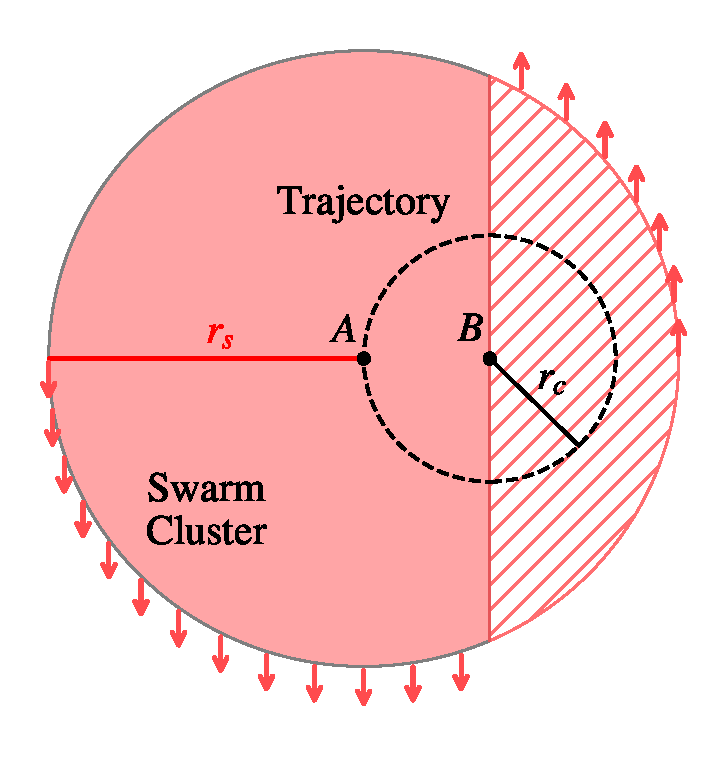
\includegraphics[width=0.6\textwidth]{./figs/rsProofEps.pdf}
%     \caption{
%         \label{fig:rsProofEps} The schematic plot of $r_s>r_c$.
%     }
% \end{figure}

\end{document}